This last section shows the characterization of the active shield (cosmic veto), which was carried out using PMTs as photosensors. Measurements of the cosmic veto using SiPM arrays has already started and their replacement will be as soon as possible. 

First, the quality of the veto coverage, shown in Figure \ref{fig:LayersVeto}, is verified. This study is done at the level of one detector so the configuration of the electronic chain used is the one shown in Figure \ref{subfig:ElectronicConfiguraiton4PMT}. To do so, the surface of the veto is divided in 9 points, shown in Figure \ref{}, which was used as a reference to place a gamma source.

FIGURAAAA

Two different tests were made for this task:
\begin{enumerate}

\item{} The first test was used to quantify the improvement of the veto signal due to its coverage. It consists of, placing a $\ce{^{137}Cs}$ source at point 2, measuring with the veto uncovered. Then cover the veto and repeat this measure. The result is shown in Figure \ref{fig:VetoCoverageImprovement}.

\begin{figure}[h]
\centering
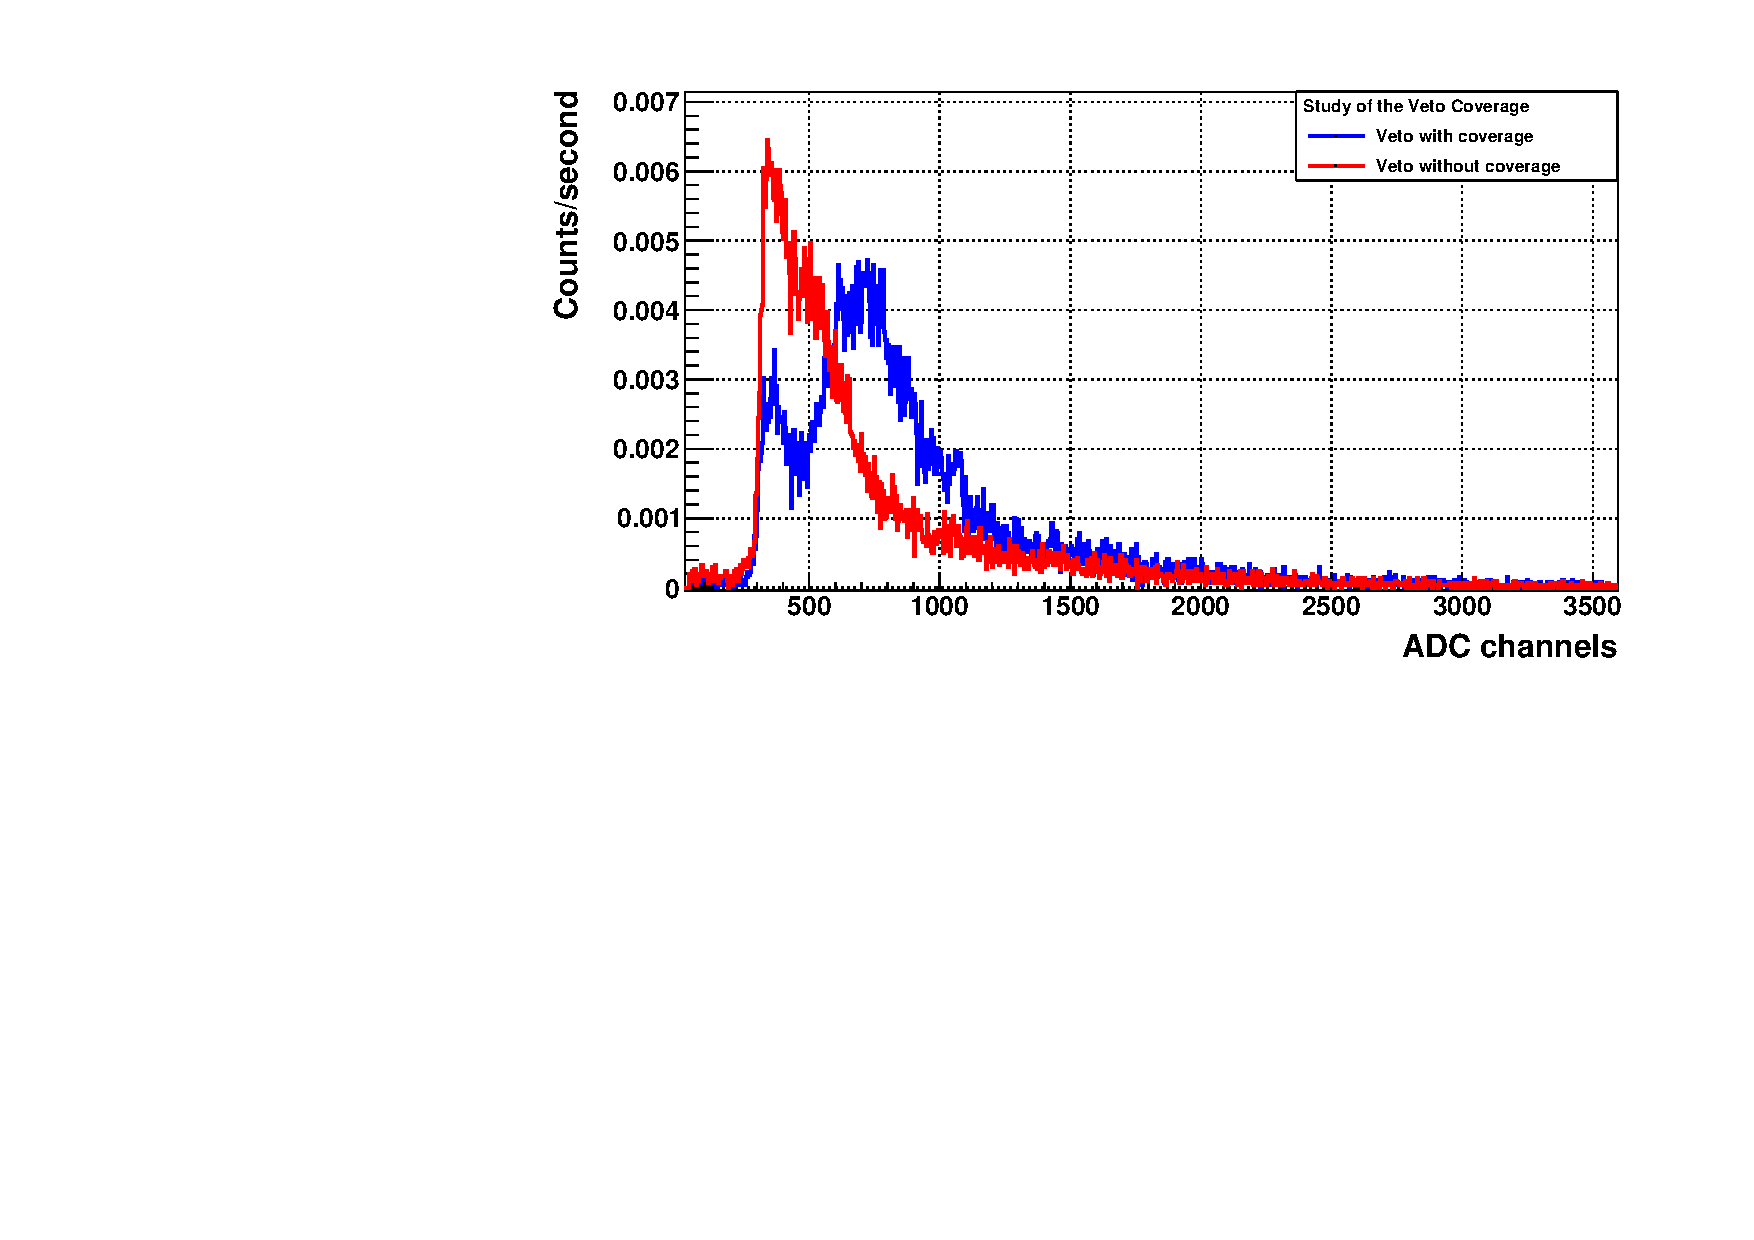
\includegraphics[scale=0.7]{4ResearchAndDevelopments/43CosmicVetos/CoverageStudy_more_rebin.pdf}
\caption{Measurement of a radioactive source $\ce{^{137}Cs}$ with the TRITIUM cosmic detector with and without its coverage.\label{fig:VetoCoverageImprovement}}
\end{figure}

It can be seen that the spectrum has shifted to the right, which means that more photons have been collected per event. No improvement was measured in the number of events detected, only an improvement in their collection efficiency.

%a comparison is made between the measurement of cover and uncover veto, placing the gamma source in 3 different points, 1, 2 and 3. This study is used 

\item{} The second test was used to verify the spatial uniformity of the signal in the covered veto. For this task, a mapping was carried out, which consists of placing a $\ce{^{60}Co}$ source at each point and measure the number of events detected in the same time windows (). It was done for two different veto and the energy spectrum obtained was integrated. The number of count rate obtained in each point is displayed in Table \ref{tab:MappingDataVetos} for both vetos, the values of which is represented in a bidimensional plot in Figures \ref{} and \ref{}, respectively.

\begin{table}[htbp]
%%\centering
\begin{center}
\begin{tabular}{|c|c|c|}
\hline
Point & Veto 1 (counts/s) & Veto 2 (counts/s)\\
\hline \hline \hline
1 & $18028\pm 3$ & $18293 \pm 1.5$ \\ \hline
2 & $19133 \pm 5$ & $20014 \pm 4$  \\ \hline
3 & $17858 \pm 4$ & $18843 \pm 4$  \\ \hline
4 & $18969 \pm 5$ & $18761 \pm 5$  \\ \hline
5 & $19893 \pm 4$ & $19841 \pm 3$  \\ \hline
6 & $18573 \pm 4$ & $18850 \pm 5$  \\ \hline
7 & $18200 \pm 4$ & $17790 \pm 4$  \\ \hline
8 & $19725 \pm 4$ & $19312 \pm 4$  \\ \hline
9 & $18030 \pm 5$ & $17804 \pm 5$  \\ \hline
\end{tabular}
\caption{Count rate measured with two different cosmic detectors using a radioactive source $\ce{^{60}Co}$.}
\label{tab:MappingDataVetos}
\end{center}
\end{table}

\begin{figure}[]
 \centering
  \subfloat[Mapping of the first TRITIUM cosmic detector.]{
   \label{subfig:MappingVeto1}
    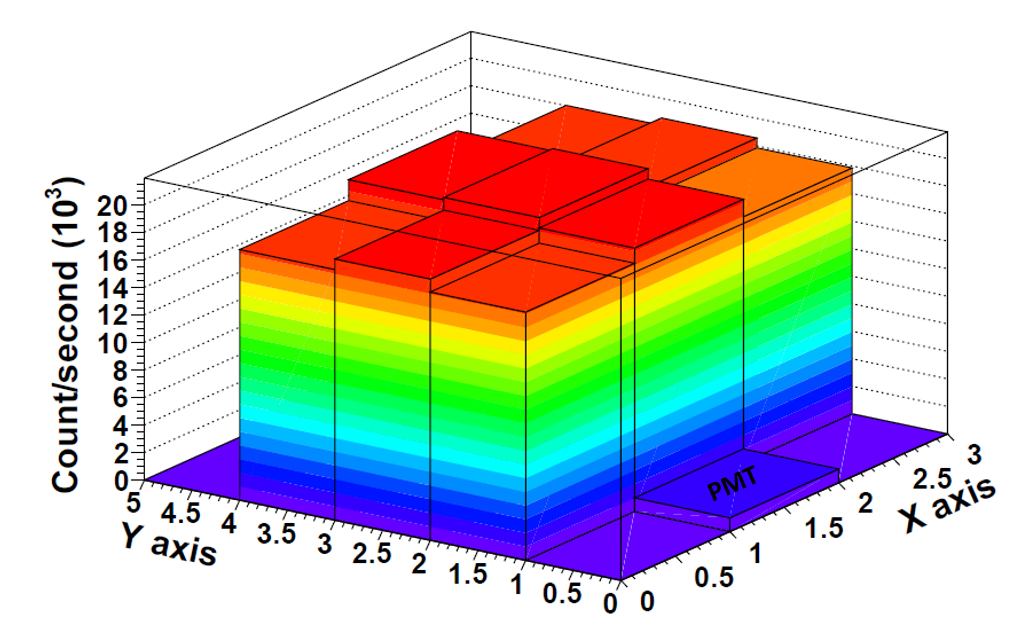
\includegraphics[width=0.9\textwidth]{4ResearchAndDevelopments/43CosmicVetos/MappingVeto1.png}}
    \newline
  \subfloat[Mapping of the second TRITIUM cosmic detector.]{
   \label{subfig:MappingVeto2}
    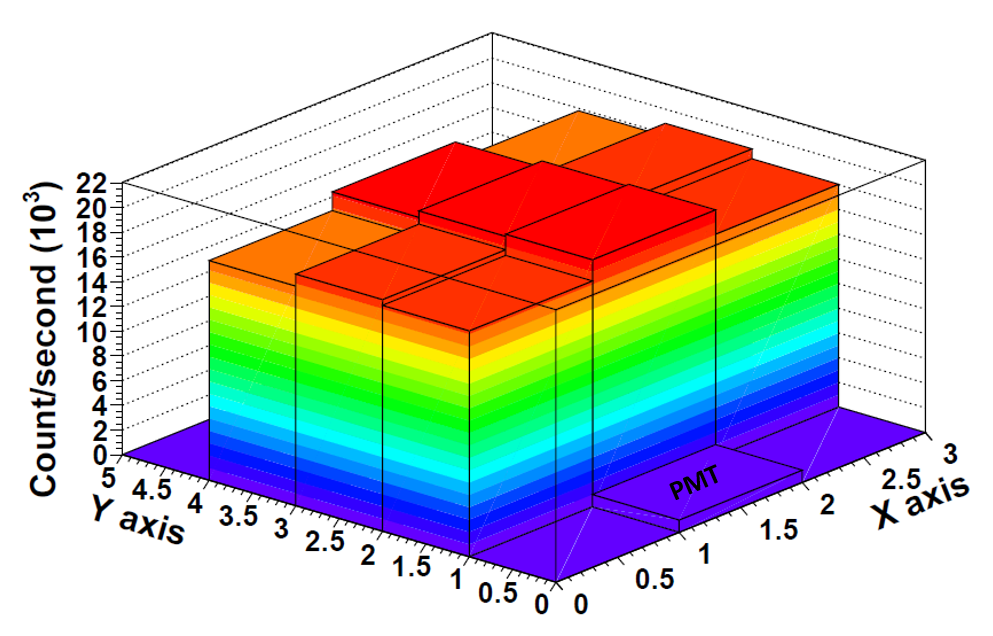
\includegraphics[width=0.9\textwidth]{4ResearchAndDevelopments/43CosmicVetos/MappingVeto2.png}}
 \caption{Bidimensional graph of the count rate (Mapping) measured with two different TRITIUM cosmic detectors using a radioactive source of  $\ce{^{60}Co}$.}
 \label{fig:MappingVetos}
\end{figure}

%EXPLICAR QUE LA PRIMERA Y ULTIMA FILA DEL PLOT BIDIMENSIONAL ES PARA PONER EL PMT.
It can be observed that the veto signal has a uniform behavior on its surface, obtaining a fairly similar counting rate in all the points considered in this study.

\end{enumerate}

The following studies of this section is done at the level of a cosmic veto (both detectors in coincidence), so the configuration of the electronic chain used is the one shown in figure \ref{subfig:ElectronicConfiguraiton4PMT}.

With the coverage of the veto correctly tested, the following step is to find the conditions in which the detection of cosmic events is optimized. This optimization consists of, on the one hand, finding the minimum high voltage of PMTs in which their efficiency is stable, and, on the other hand, finding the maximum threshold of the discriminator\footnote{The threshold is the voltage value that the PMT output signals must exceed to contribute to the cosmic detection} at which we start to loss cosmic events in their detection. For higher high voltage and smaller thresholds of the found values, a plateau should be found.

To find both parameters, two different studies were carried out, in which the number of coincident events (cosmic events) were measured. On the one hand, it was measured at several high voltages and fixed thresholds and, on the other hand, it was measured at several thresholds and fixed high voltages. Both measurements are shown in Figure \ref{fig:HVandThresholdsPLateaus} in which a semi-logarithmic scale is used.

To find the optimized conditions the amplification line of the configuration of the electronic chain \ref{subfig:ElectronicConfiguraiton4PMT} was eliminated and the output signal of the coincidence module, second stage, was connected to a CAEN Quad Scaler And Preset Counter-Timer module, N. 1145, \cite{ScalerDataSheet}, used to count the number of events in a time window of $300~\second$.

\begin{figure}[]
 \centering
  \subfloat[Counts per second for several high voltage at three different thresholds.]{
   \label{subfig:HVPLateauVetos}
    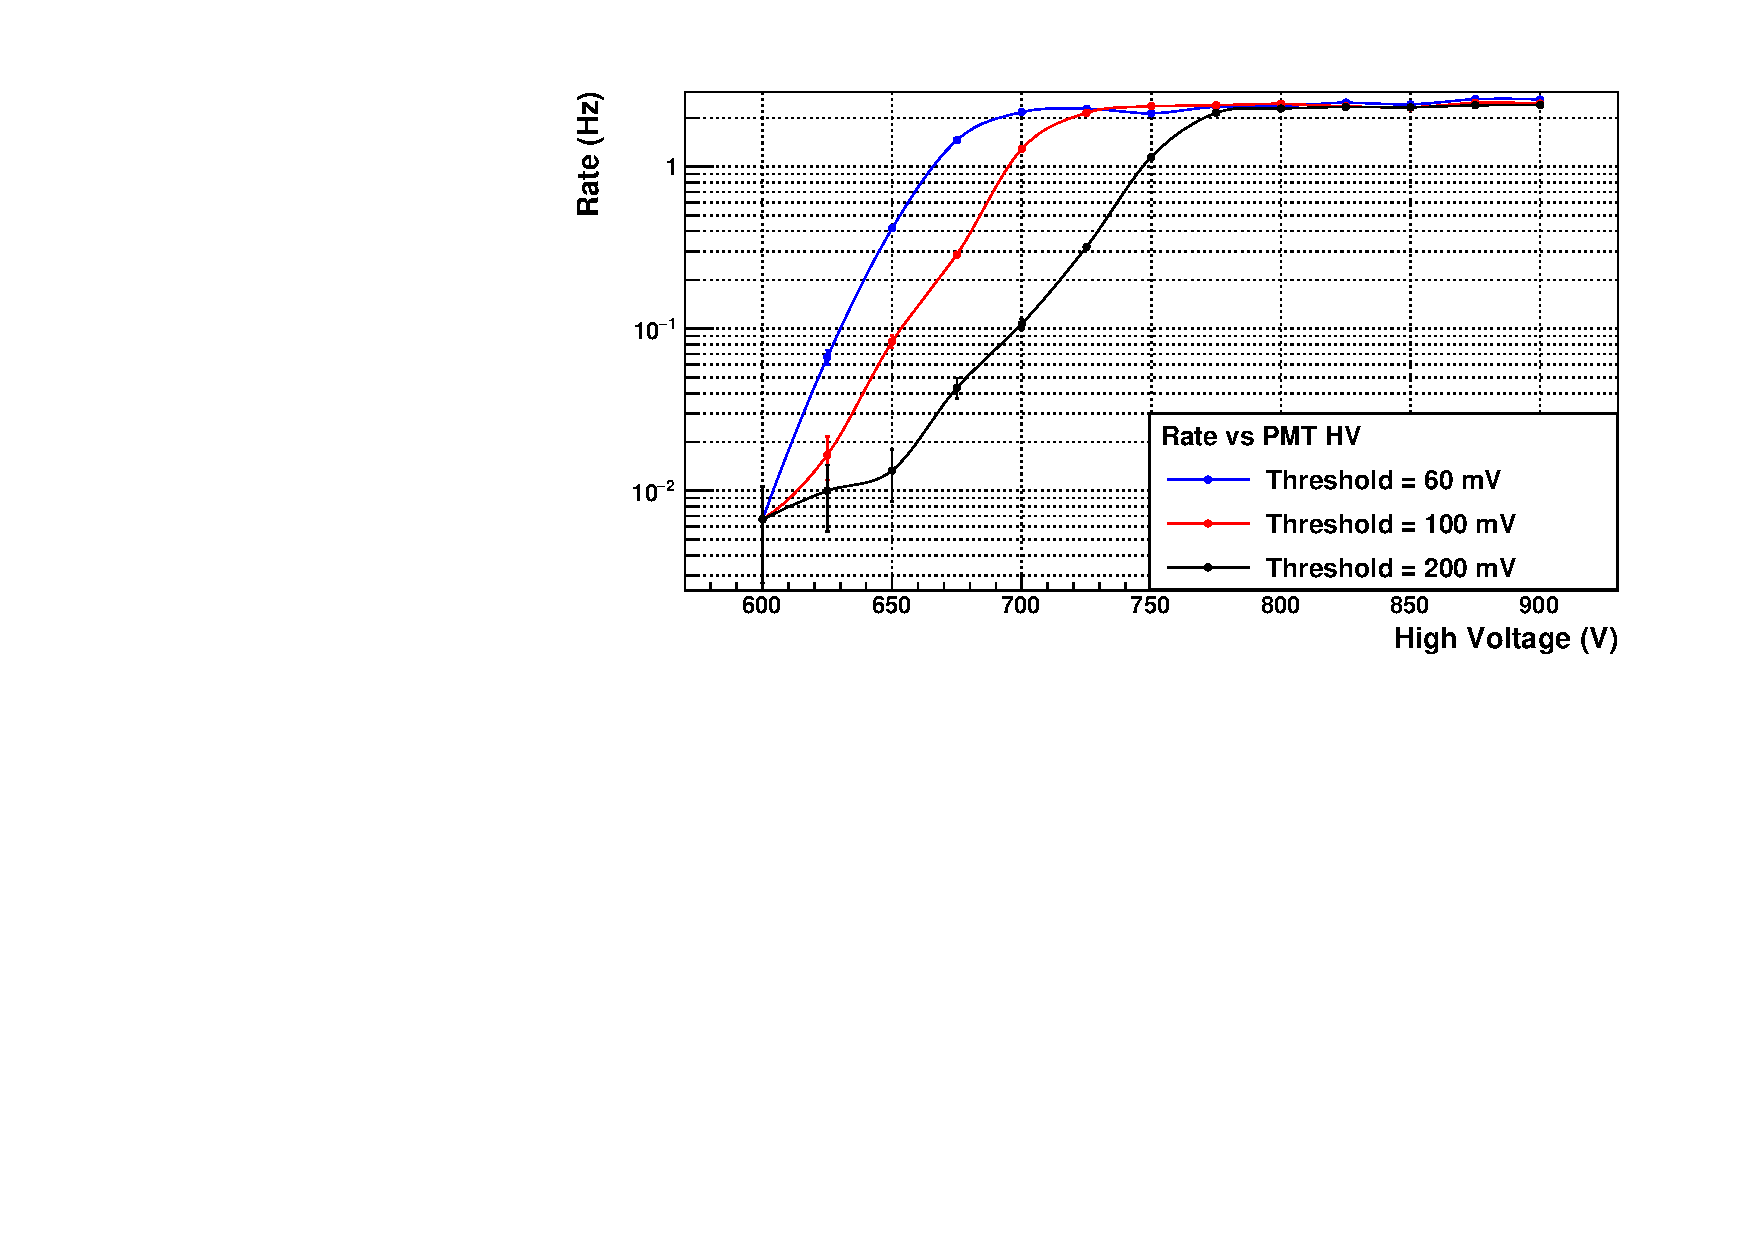
\includegraphics[width=0.8\textwidth]{4ResearchAndDevelopments/43CosmicVetos/Counts_for_several_HV_VETOS.pdf}}
    \newline
  \subfloat[Counts per second for several thresholds at three different high voltage.]{
   \label{subfig:ThresholdsPlateau}
    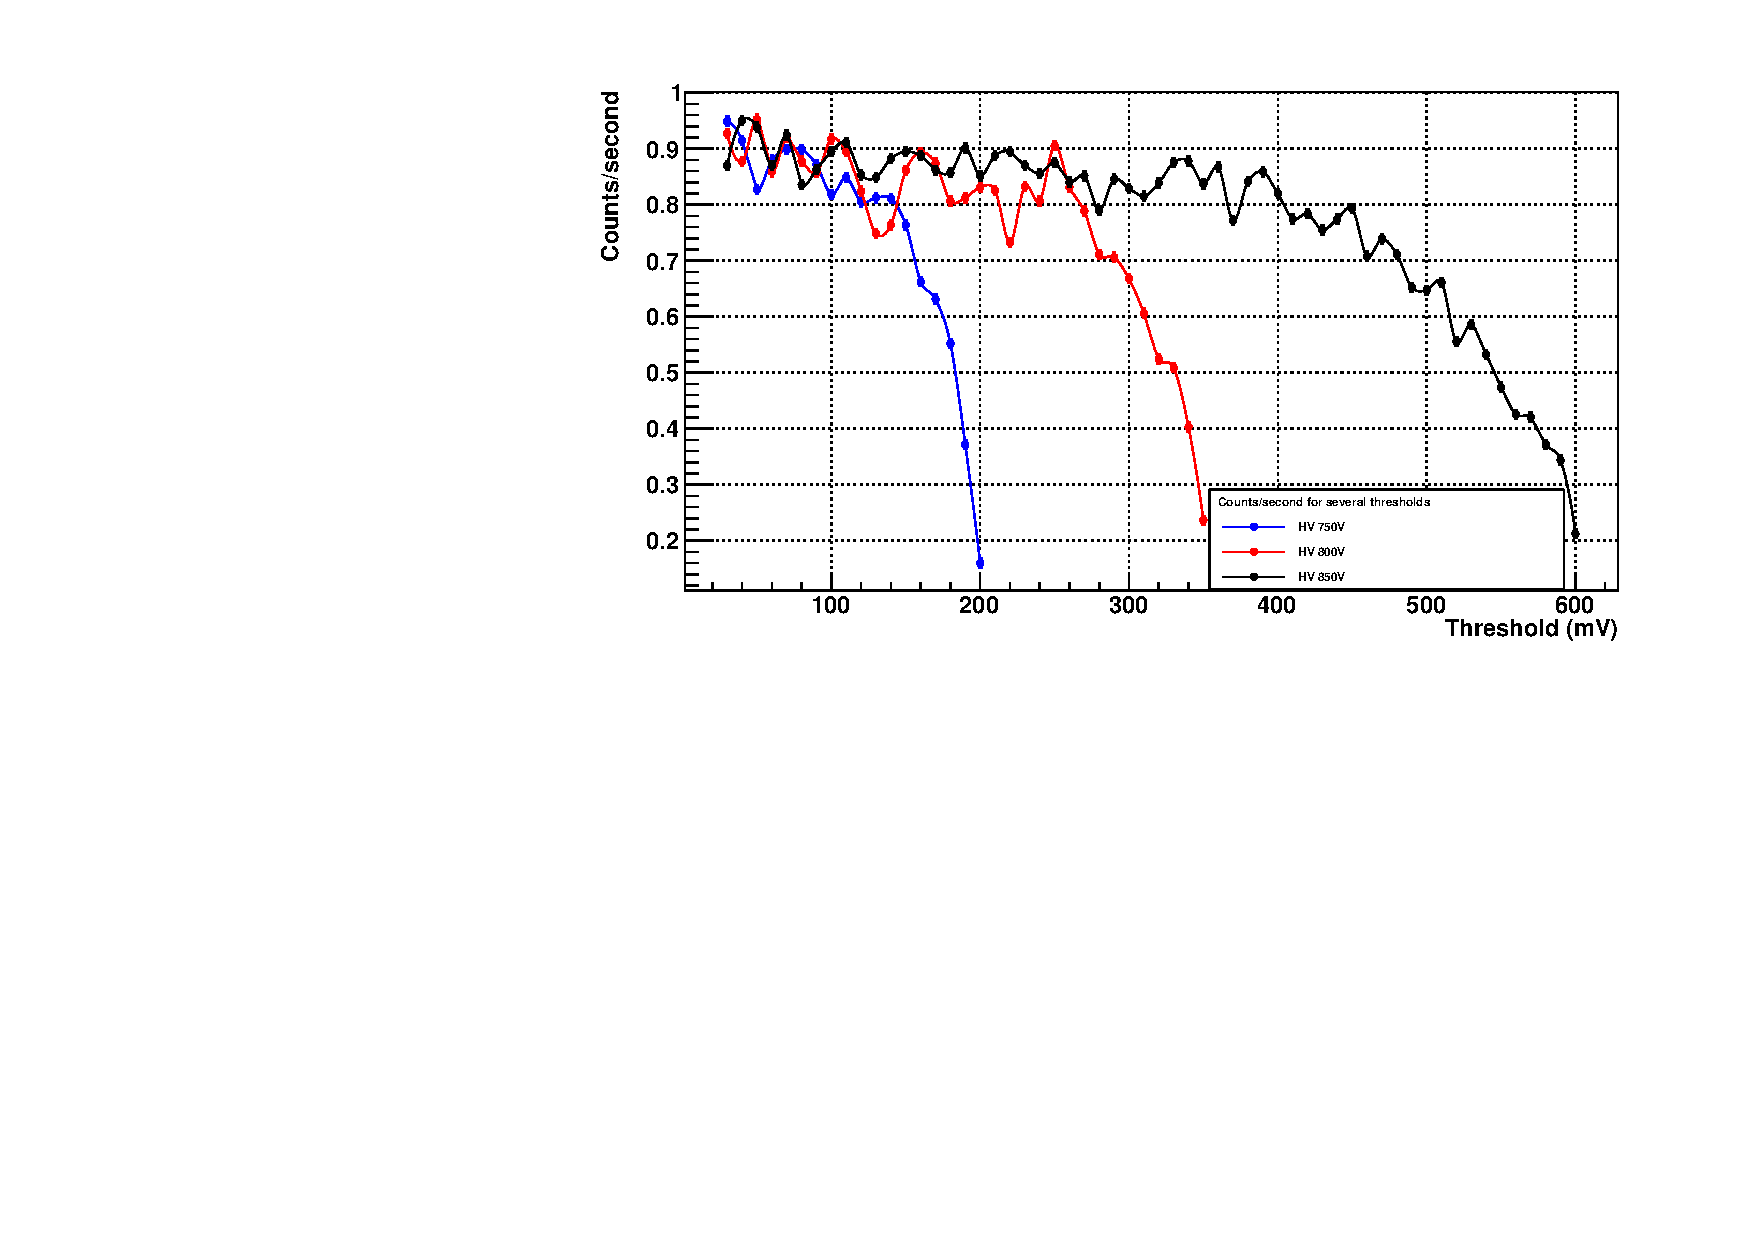
\includegraphics[width=0.8\textwidth]{4ResearchAndDevelopments/43CosmicVetos/Counts_for_several_thresholds_VETOS.pdf}}
 \caption{Counts per second at several high voltage and fixed thresholds and several thresholds and fixed high voltage.}
 \label{fig:HVandThresholdsPLateaus}
\end{figure}

In Figure \ref{subfig:HVPLateauVetos}, the measurements at several high voltage and a fixed thresholds is shown, which was done for three different thresholds, $60~\milli\volt$, $100~\milli\volt$ and $200~\milli\volt$. As can be seen, there is a minimum high voltage for each threshold used, $700~\volt$, $730~\volt$ and $780~\volt$ respectively, at which the plateau start. This minimum voltage is higher when the value of the threshold is increased, as it should happen. The voltage chosen to work is $800~\volt$ since it can be assured that it is on the plateau for the three thresholds.

In the same way, in Figure \ref{subfig:ThresholdsPlateau}, the measurements at several thresholds and a fixed high voltage is shown, which was done for three different high voltages, $750~\volt$, $800~\volt$ and $850~\volt$. As can be seen, there is a maximum threshold for each high voltage used,  $140~\milli\volt$, $270~\milli\volt$ and $450~\milli\volt$ respectively, at which the plateau ends. This maximum threshold is increased for higher voltage, as it should happened. The threshold choosen to work is $200~\milli\volt$ since, for the previous election, $800~\volt$, it can be sure of being on the plateau. 

Next, the energy spectrum of cosmic events was measured, which is shown in Figure \ref{fig:EnergySpectrumCosmicVeto}. For this task the configuration of the electronic chain shown in Figure \ref{subfig:ElectronicConfiguraiton4PMT} was used with the values previously mentioned, $800~\volt$ and $200~\milli\volt$. 

\begin{figure}[h]
\centering
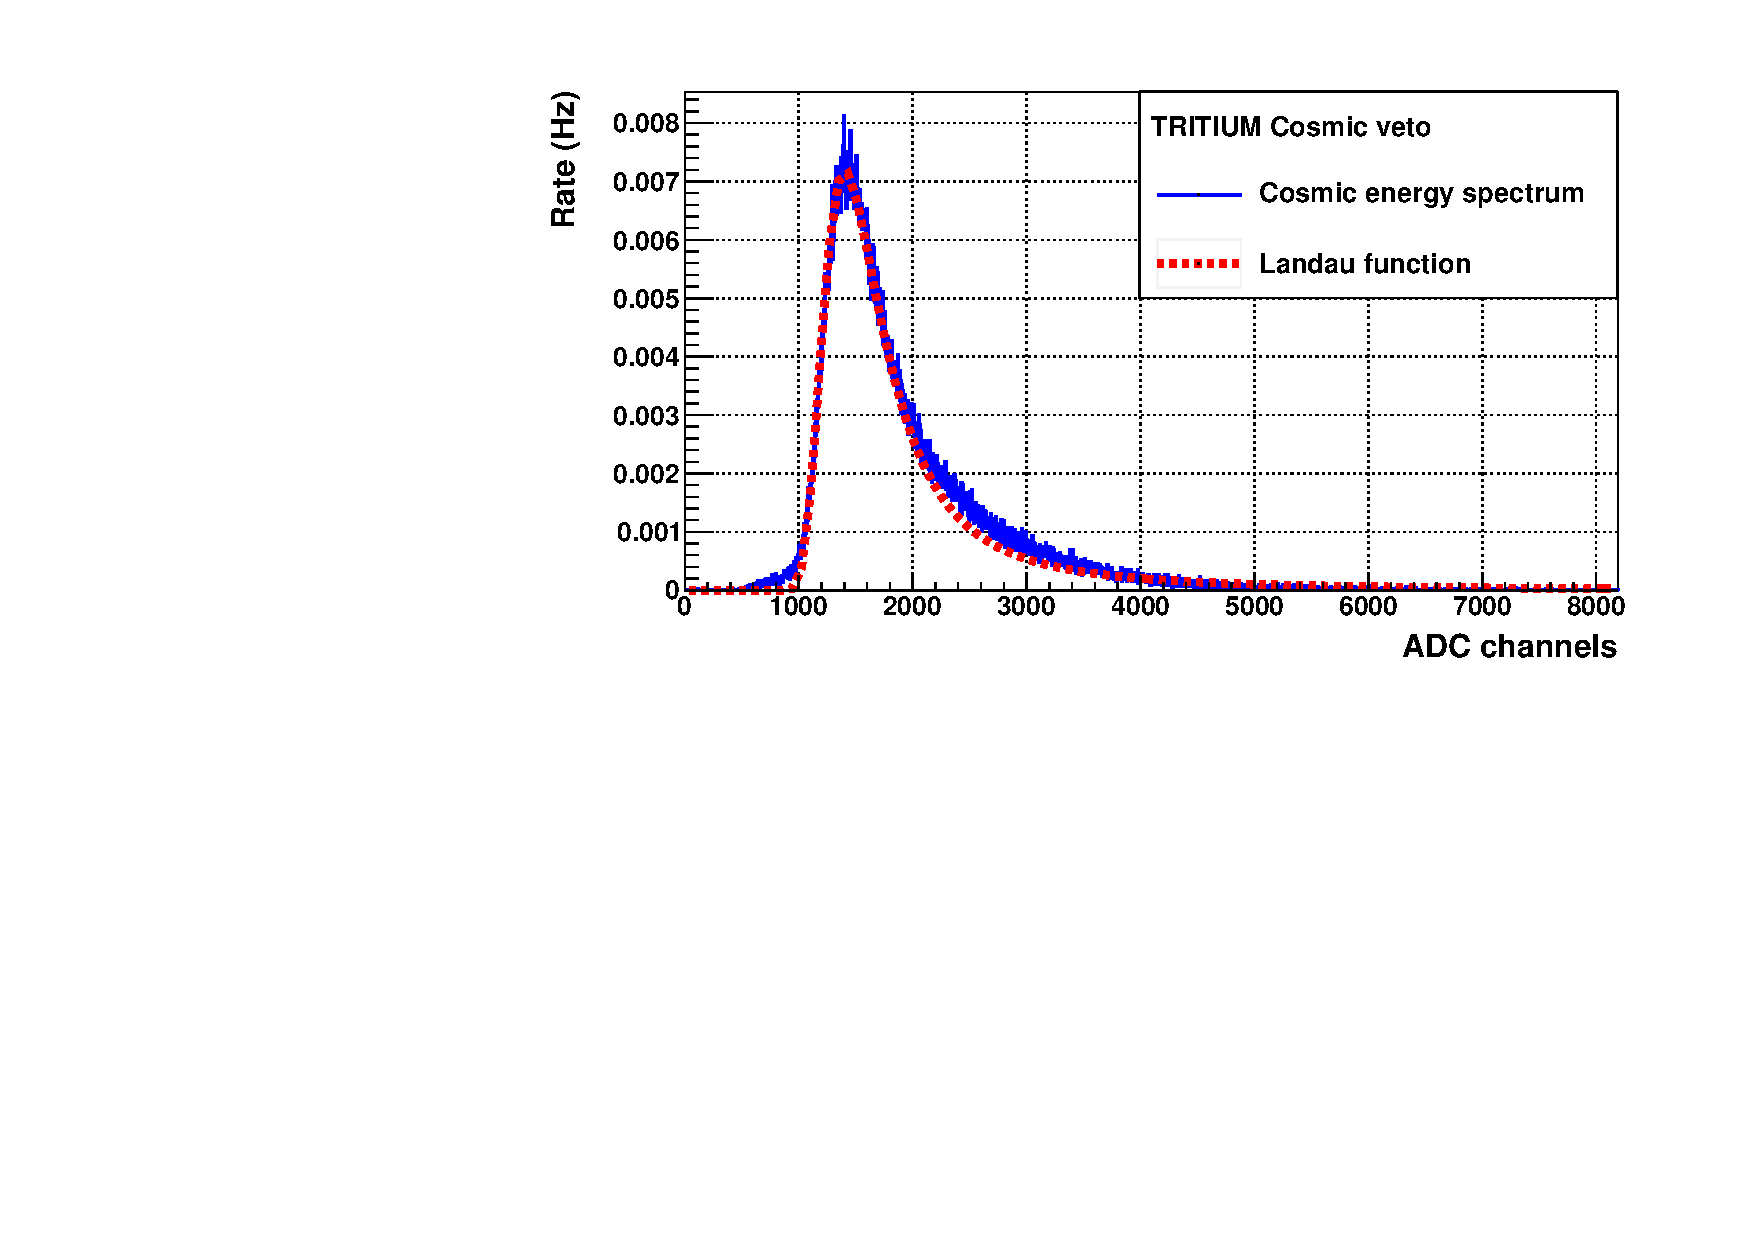
\includegraphics[scale=0.6]{4ResearchAndDevelopments/43CosmicVetos/Cosmic_Energy_Spectrum_36_cm_Landau_Function.pdf}
\caption{Energy spectrum measured with the cosmic veto.\label{fig:EnergySpectrumCosmicVeto}}
\end{figure}

As can be seen, this energy spectrum fits well with a landau function as expected. The number of detected cosmic events can be known by calculating the area integral of this spectrum, whose result is $2,5~$event$/\second$. The theoretically expected cosmic rate, calculated in section \ref{subsec:SetUpActiveShield}, is $2,909~$event$/\second$, so the efficiency of the active veto developed in TRITIUM experiment for cosmic events deteccion is $85\%$, which is a common value of the efficiency of cosmic detectors.

Finally the relationship between the detected cosmic events and the distance between both detectors that form the cosmic veto was obtained. It is interesting because this distance can be changed if other tritium prototypes are used and we need to know the expected cosmic rate for each different situation. To do so, an energy spectrum was measured for five different distances, which are approximately $10~\cm$, $20~\cm$, $36~\cm$, $40~\cm$ and $50~\cm$, which is shown in Figure \ref{subfig:EnergySpectrumsSeveralDistanceVeto}. The energy spectrum previously shown in Figure \ref{fig:EnergySpectrumCosmicVeto} was also included. 

%\begin{figure}[]
%\centering
%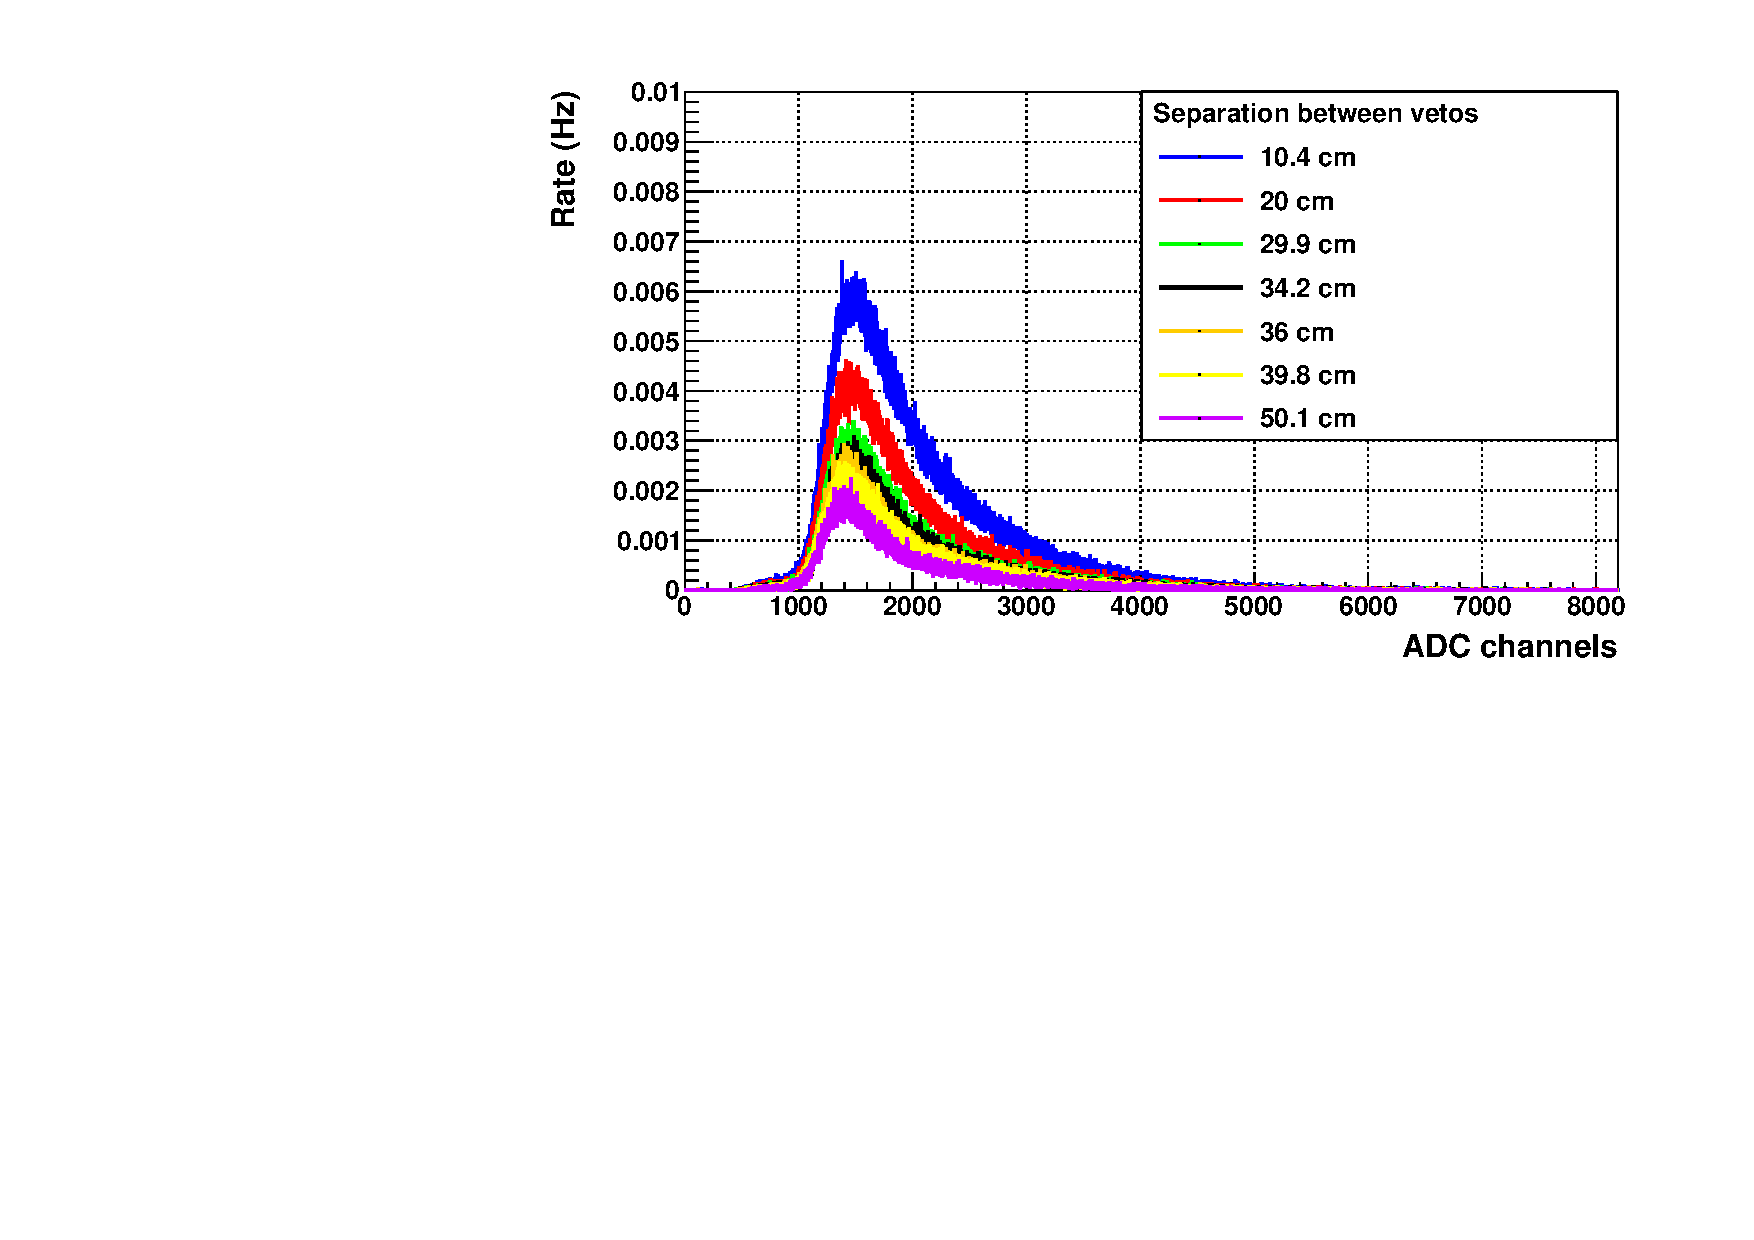
\includegraphics[scale=0.6]{4ResearchAndDevelopments/43CosmicVetos/Energy_Plots_SeveralDistance_Veto.pdf}
%\caption{Energy spectrum of cosmic vetos for several distance between cosmic detectors.\label{fig:EnergySpectrumsSeveralDistanceVeto}}
%\end{figure}

As we can see, the shape of the spectrum is the same because the energy of the detected events is the same (cosmic events) but the quantity of their events is less for greater distance. The reason for that is that when we increase the distance, the solid angle formed by the active veto is smaller.

The detected cosmic events was calculated by the area integral and they are represented in Figure \ref{subfig:LinearFitSeveralDistanceVeto} as a function of the distance between both detectors, where a linear fit has been added. With this linear fit, the detected cosmic rate can be easily known if the working distance is changed. 

%\begin{figure}[htbp]
%\centering
%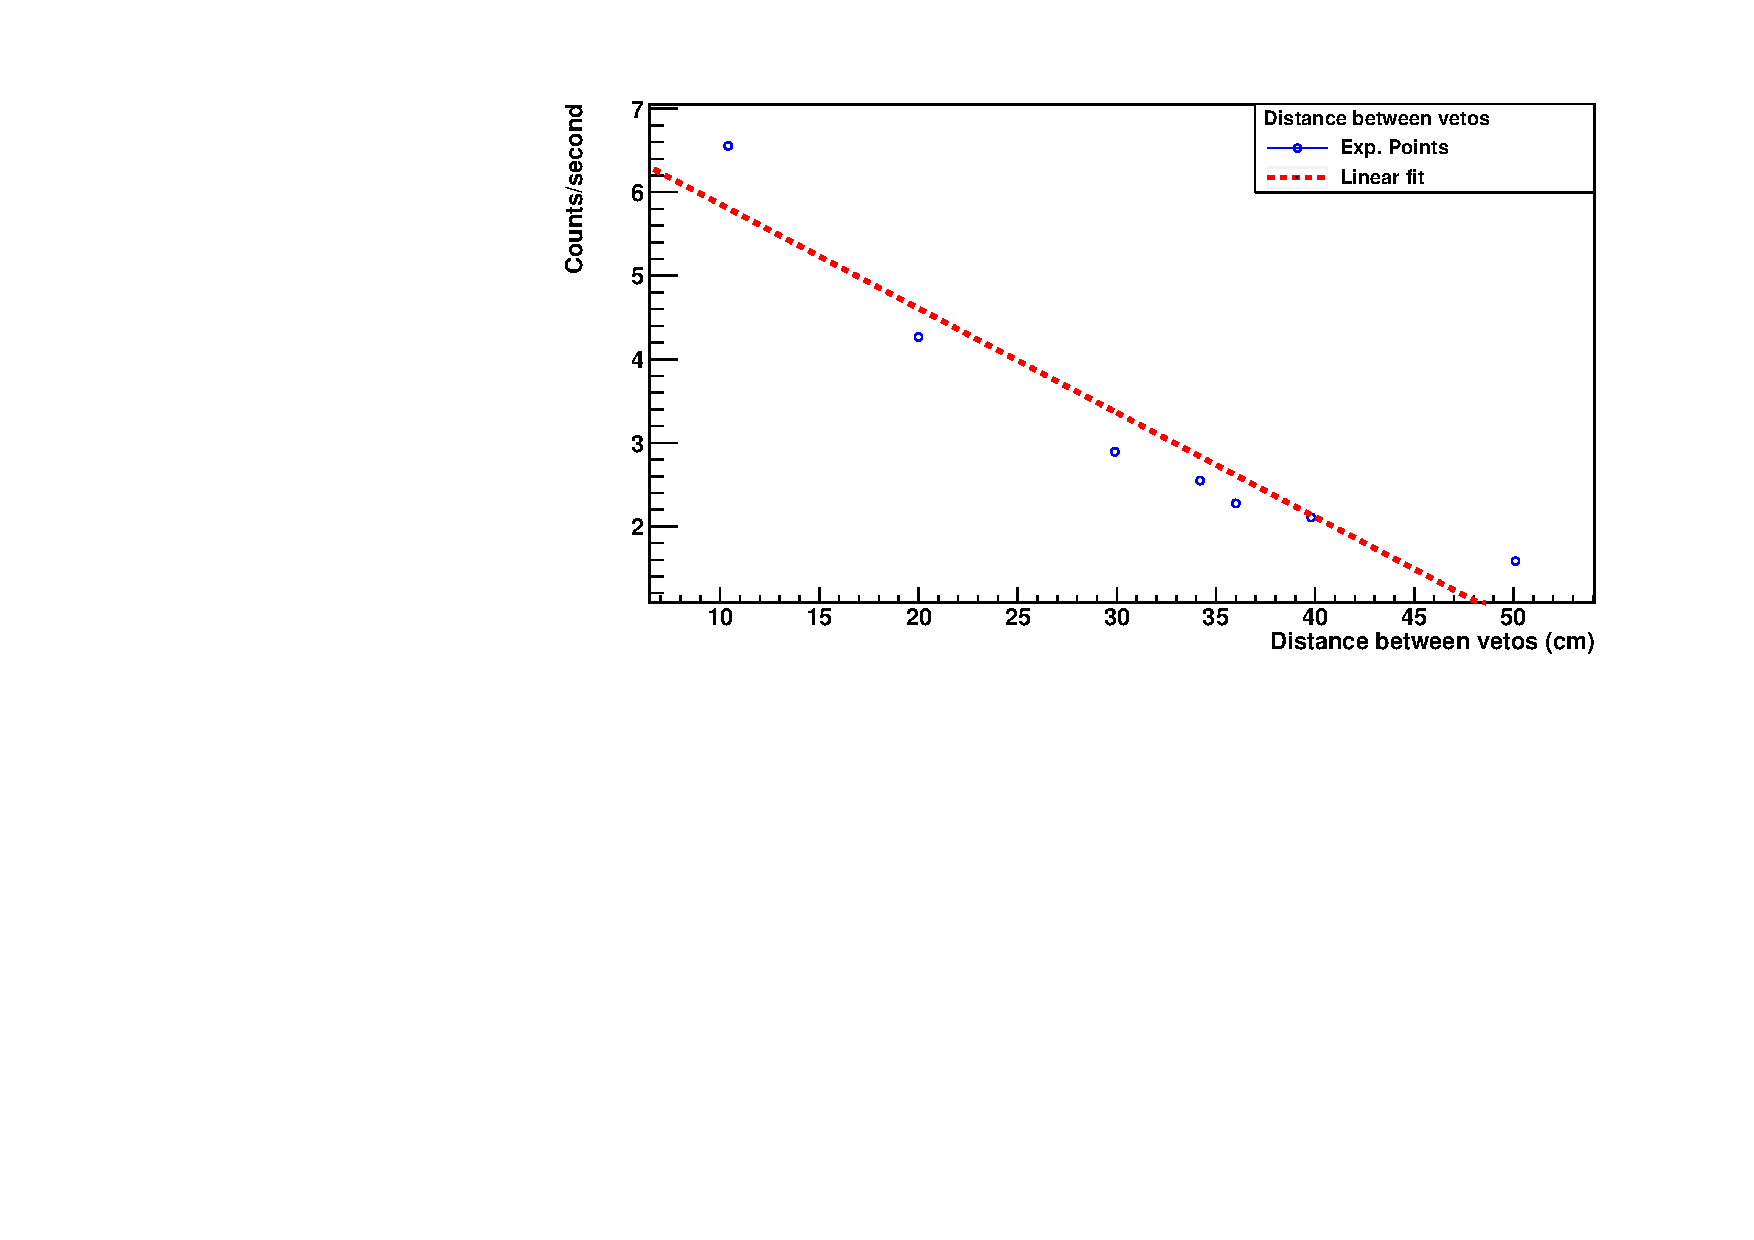
\includegraphics[scale=0.6]{4ResearchAndDevelopments/43CosmicVetos/LinearFit_SeveralDistance_Veto.pdf}
%\caption{Linear fit of the counts per second measured with the cosmic veto with several distance between its cosmic detectors.\label{fig:LinearFitSeveralDistanceVeto}}
%\end{figure}


\begin{figure}[htbp]
 \centering
  \subfloat[Energy spectrum of the cosmic veto for several distance.]{
   \label{subfig:EnergySpectrumsSeveralDistanceVeto}
    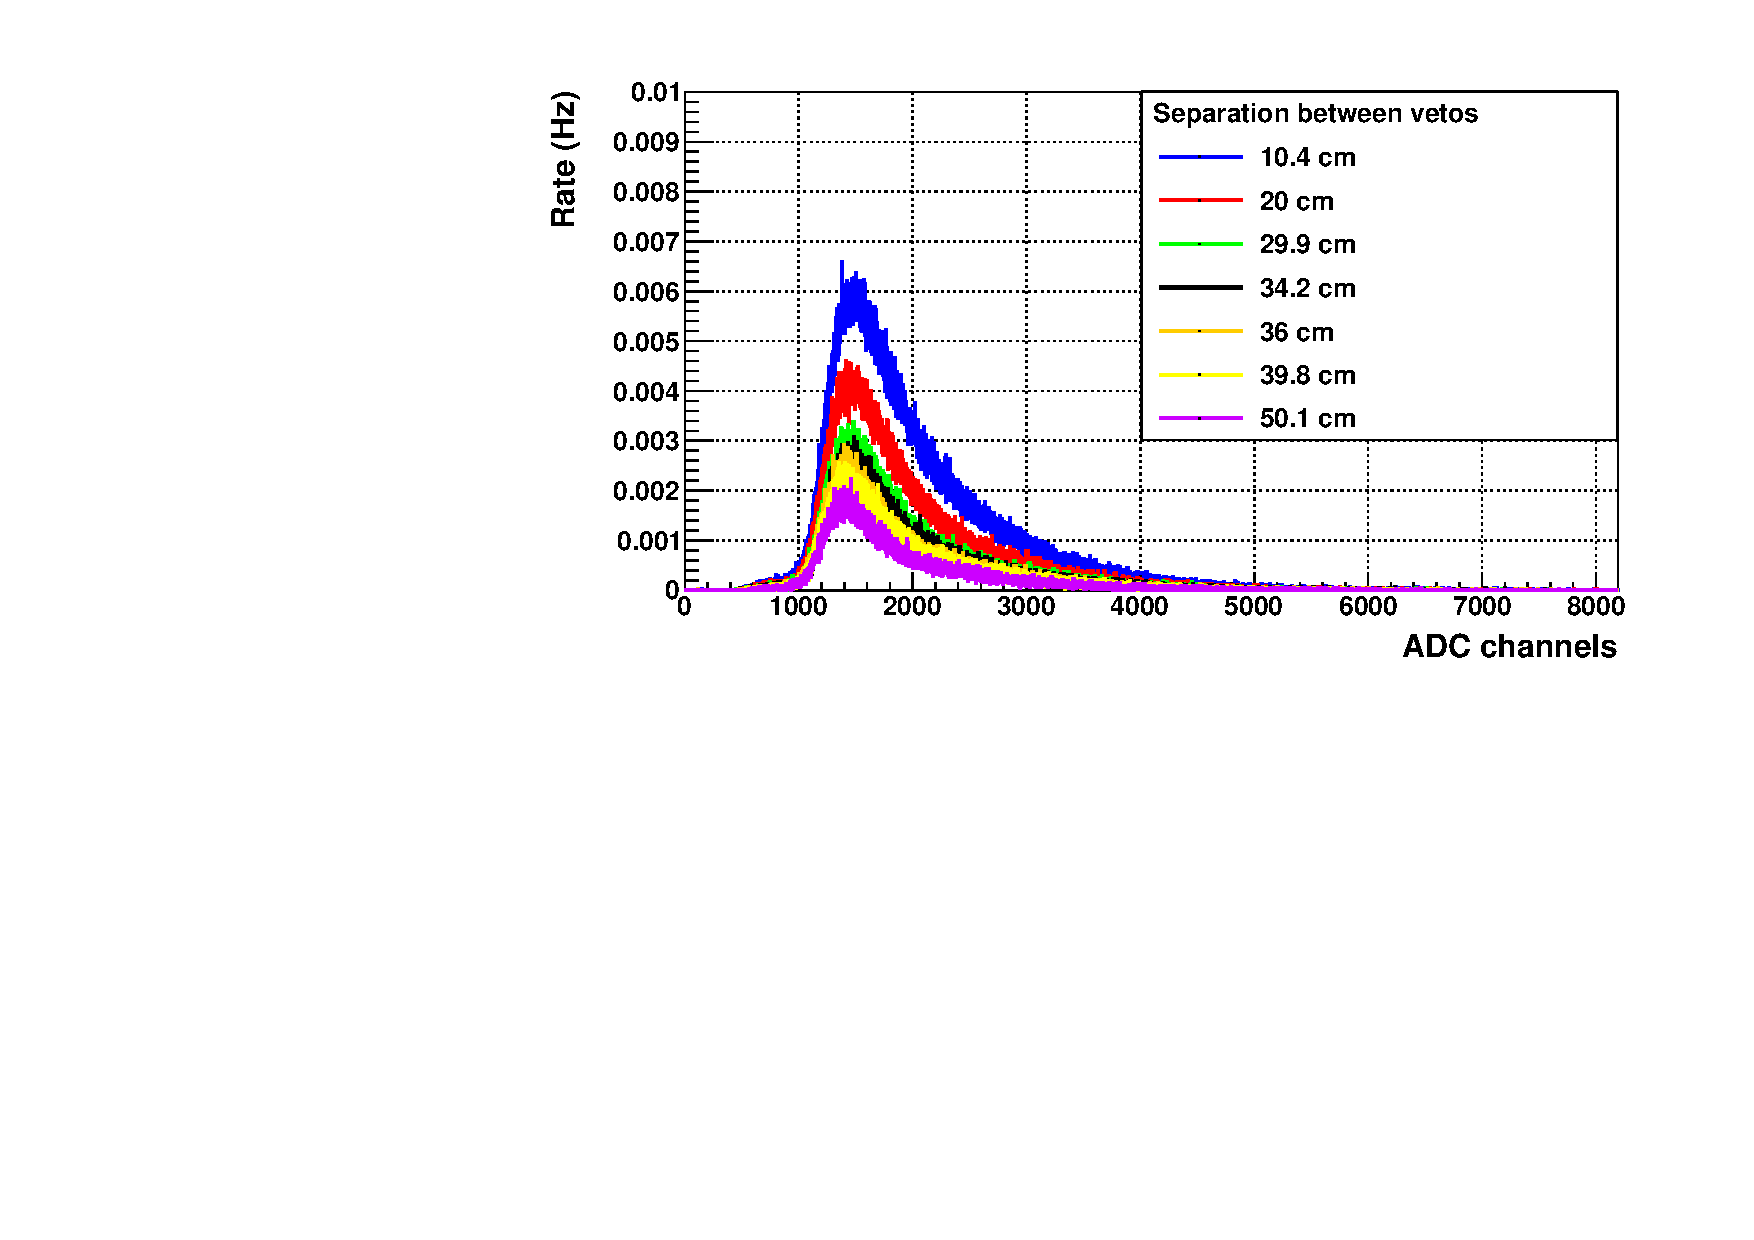
\includegraphics[width=0.85\textwidth]{4ResearchAndDevelopments/43CosmicVetos/Energy_Plots_SeveralDistance_Veto.pdf}}
    \newline
  \subfloat[Linear fit of counts per second measured with the cosmic veto for several distance.]{
   \label{subfig:LinearFitSeveralDistanceVeto}
    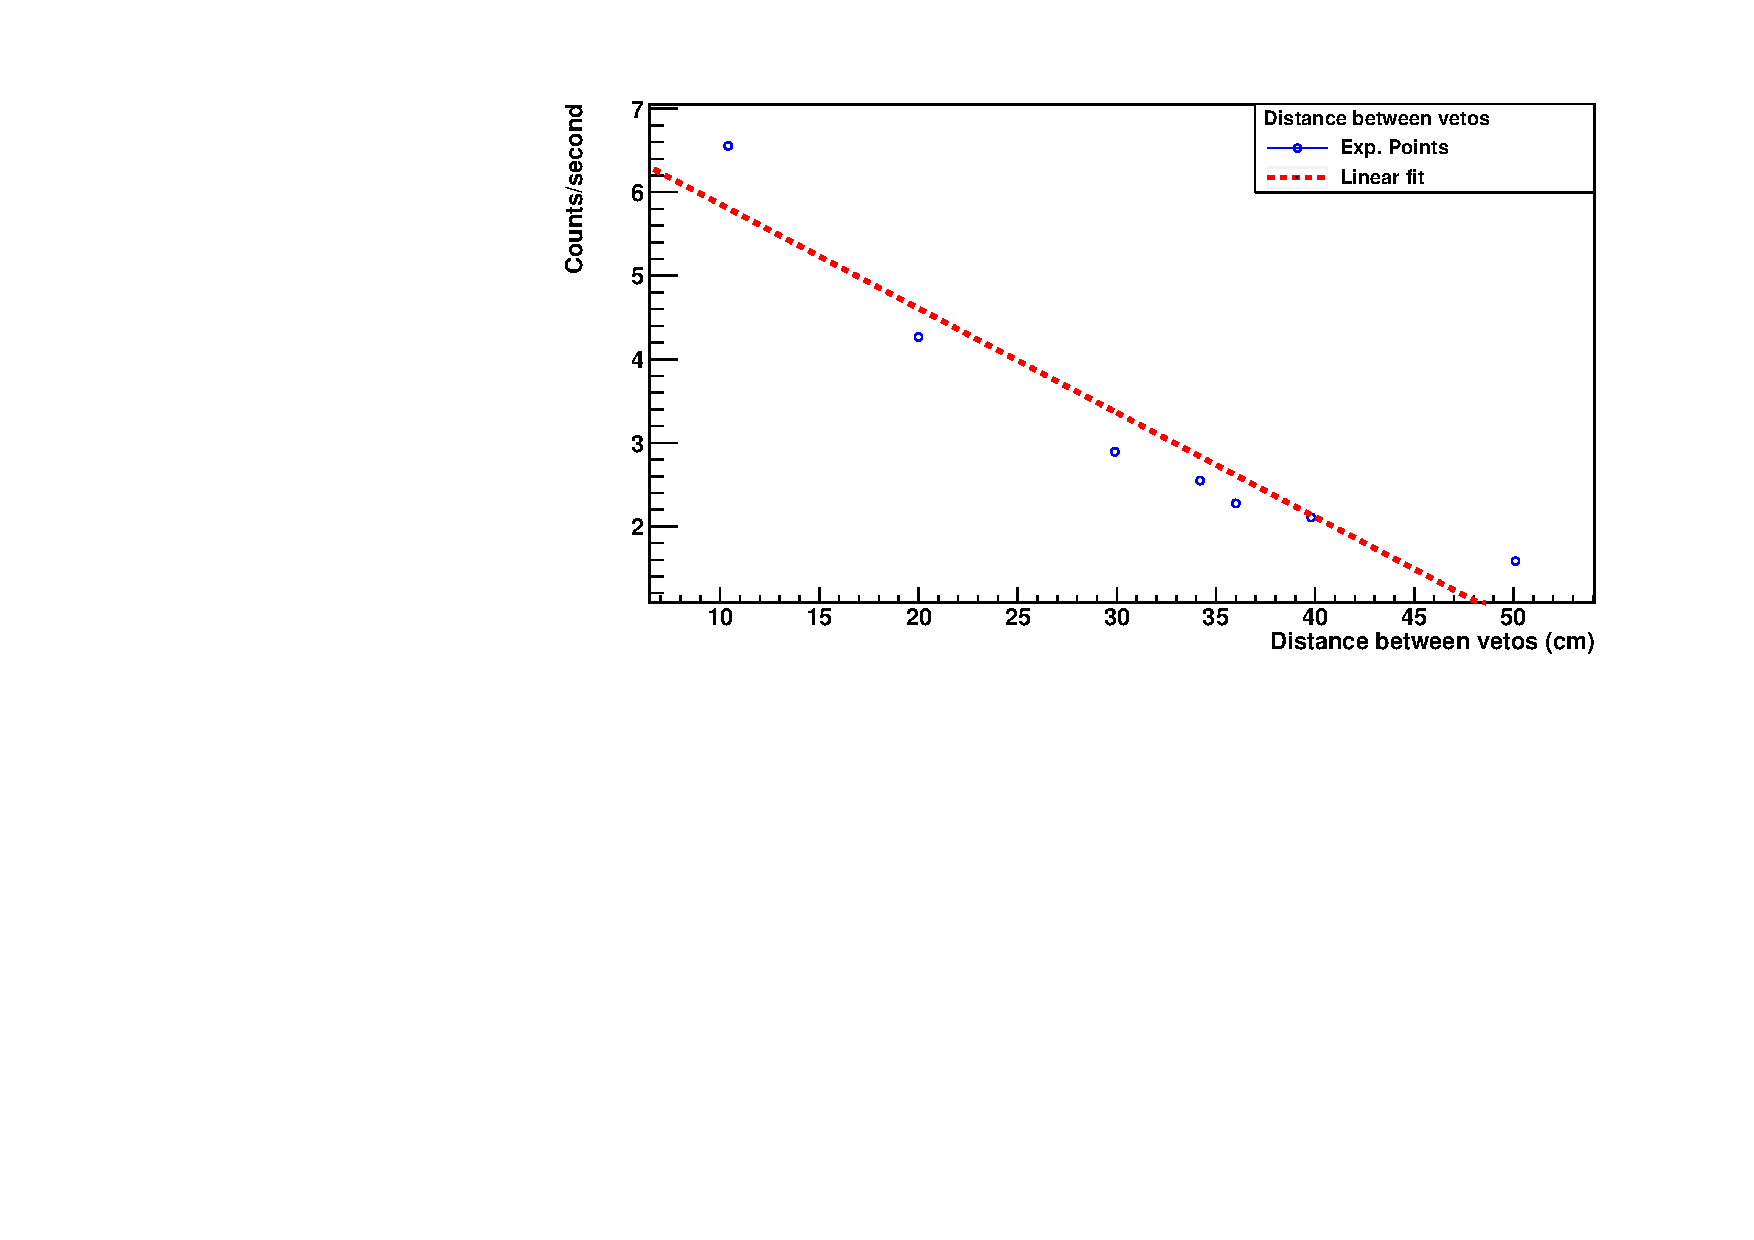
\includegraphics[width=0.85\textwidth]{4ResearchAndDevelopments/43CosmicVetos/LinearFit_SeveralDistance_Veto.pdf}}
 \caption{Measurement of the cosmic veto for several distances between its cosmic detectors.}
 \label{fig:DistanceVeto}
\end{figure}


%También se realizaron varias medias para ver como afecta una fuente gama. Discutir con Pepe como plantear esta medida o si merece la pena ponerla o no.

%Como es de esperar esta deja muy poca señal en el centelleador ya que este tiene muy poca eficiencia para gammas.